\chapter{Casebeskrivelse}
\label{chp:case}

OVERGANG RIT -> ST.OLAVS OG INNFØRING AV SYSTEMET
Pasientsignalsystemet som brukes ved St.Olavs Hospital i dag, ble innført da det ble bygget nytt sykehus i \textbf{????}. 

\noindent
ARKITEKTUR
Når det skulle bygges nytt sykehus ble utformingen av avdelingene endret. Avdelingene fikk flere sengeposter som igjen er delt i sengetun, hvor hvert sengetun normalt har seks til åtte pasientrom. Sengetunet er en fysisk og funksjonell måte å organisere pasientrommene på, og for å sikre fleksibilitet og effektivitet ligger flere sengetun ved en sengepost etter hverandre i serie, som vist i figur \ref{fig:sengepost}. Signalsystemet kan til en viss grad konfigureres på en slik måte at sykepleiere på et sengetun kan motta pasientsignaler fra andre sengetun \citep{Aslaksen}.

FORSKJELL PÅ A1 OG A2/A3

\begin{figure}[H]
\centering
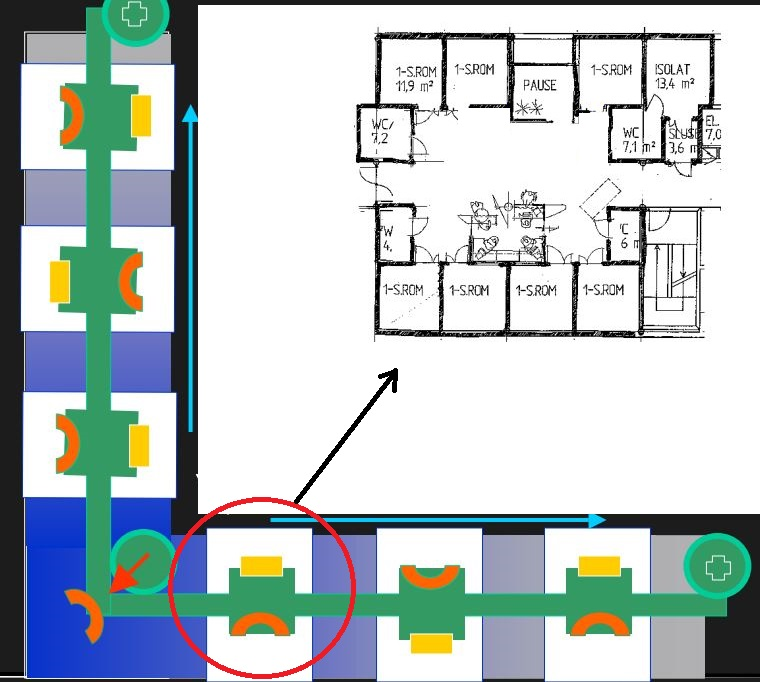
\includegraphics[scale=0.3]{sengepost.jpg}
\caption{Sengepost inndelt i sengetun \citep{Aslaksen}}
\label{fig:sengepost}
\end{figure}

\noindent
Sammen med planleggingen av nytt sykehus ble det også planlagt ny infrastruktur. Det ble satt opp overodnede krav til systemet, og da ingen av rådgiverende i helsebygg turte å ta risikoen med et slikt innovativt system ble oppdraget lagt ut for anbud. Firmaet IMATIS ble gründet på bakgrunn av dette, og hadde med seg erfaring fra olje- og prosessindustrien. De utviklet et konsept basert på de som blandt annet brukes overvåke produksjon på oljeplatformer, med en meldingstjener i bunnen, og et trådløst system som bygger på det. De fikk med seg en $"$vanlig$"$ pasientsignalleverandør, BEST, til å lage grensesnittet til systemet. 

\noindent
Det nye systemet ble innført etterhvert som avdelingene flyttet inn i sine nye bygg. De ansatte ble sendt på dagskurs i forkant av dette, hvor halve dagen var viet til opplæring i systemet. Noen ansatte fikk mer omfattende opplæring, og ble superbrukere av systemet. Den første tiden etter at systemet var tatt i bruk var det også plassert $"$on site help desk$"$ på alle avdelinger for å svare på spørsmål og hjelpe til med bruk. I dag er det den enkelte avdeling som har ansvar opplæring av sine nyansatte. 

\noindent
Etter innflyttingen i nytt sykehus var det meningen at alle skulle bruke telefonen til å motta pasientsignaler. Det var derimot noen avdelinger, deriblandt A1 lokalisert i nevrosenteret, som viste sterk motstand og nektet å bruke telefonene til dette.

\noindent
ER FLYTTET TIL RESULTATER
Høsten 2013 flyttet avdelingen A1 inn i nye lokaler i kunnskapsparken. I forbindelse med dette gikk de med på å bruke systemet slik det var tiltenkt i en prøveperiode på 14 dager, i håp om at dette skulle endre de negative holdningene til systemet. Etter denne prøveperioden gikk avdelingen derimot tilbake til å ikke motta pasientsignaler på telefon. 
I forbindelse med flyttingen fikk de også tilbake assistanseknappen de lenge hadde ønsket seg. Denne er plassert sammen med den grønne og røde knappen på panlet inne på pasientrommet, og brukes til å fortelle kolleger at man har behov for assistanse. Varslingen fra denne kanppen vises kun på veggpanelene og ikke på IMATISskjermen.

\section{System}
SYSTEMBESKRIVELSE OG GODTA/AVVIS
En overodnet oversikt over hvordan vasling av pasientsignal fungerer er illustrert i figur \ref{fig:detteskjer}. En mer detaljert beskrivelse er veldlagt i tillegg \ref{chp:appendix_dagenssystem}.
Pasientene kan tilkalle sykepleier blandt annet ved å trekke i snoren på anropspanelet, som er montert på veggen ved sengen. Signalet varsles da via vaktromsapparatet som henger synlig på sengetunet, og via rompaneler på de rommene hvor sykepleiere er tilstedemarkert (denne markeringen gjøres ved at sykepleier trykker på den grønne knappen på rompanelet). 
Sykepleieren med primæransvar for pasienten vil ved utløst pasientsignal bli varslet på sin trådløse enhet, en Cisco IP-telefon. 
Ved et innkommende pasientsignal kan sykepleieren velge å godta eller avvise signalet gjennom to kanpper på telefonen. Dersom velger å avvise sigalet, eller ingen valg gjøres innen 15 sekunder sendes signalet videre til neste pleier på bemanningsplanen som settes opp, og konfigureres på PC'en på sengetunet.

\begin{figure}[H]
\centering
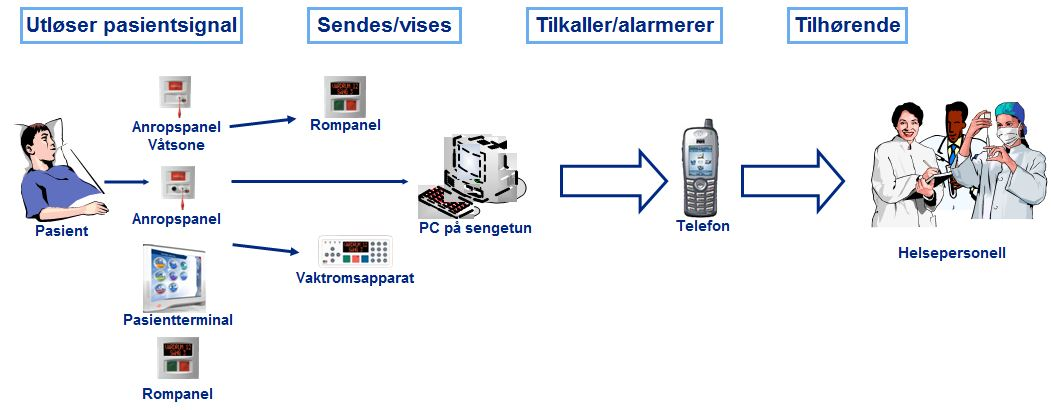
\includegraphics[scale=0.5]{alarmprosess.jpg}
\caption{Dette skjer ved utløst pasientsignal.}
\label{fig:detteskjer}
\end{figure}

\noindent
SLØYFER/UTFORMING
Vaslingssystemt består av et fast og et trådløst system, hvor det faste består av veggpanelene, mens det trådløse består av de IP-telefonene og IMATIS-systemet. Det faste systemet er konfigurert i fysiske, kablede sløyfer som kobler sammen sengetun på avdelingene og gjør det mulig å motta vaslinger fra andre tun på veggpanelene. For det trådløse systemet konfigureres dette gjennom bemanningsplanen. 


\noindent
FORSINKELSE

ARBEIDSLISTEN

TELEFON SKAL EGENTLIG VÆRE SYSTEM NUMMER 1?????

KAN VELGE PRIMÆR/DISP OSV

